\documentclass[11pt,letterpaper]{article}
\usepackage{graphicx}
\usepackage{geometry}
\usepackage{amsmath}
\usepackage{hyperref}
\usepackage{natbib}
\usepackage{booktabs}
\usepackage{xcolor}
\usepackage{url}
\usepackage{microtype}

\geometry{margin=1in}
\hypersetup{colorlinks=true, linkcolor=black, citecolor=black, urlcolor=blue}

\title{\textbf{Efficiency at a Cost: Applying the Marginal Value Theorem\\to Scientific Document Retrieval}}

\author{%
  Anonymous Author(s)
}

\date{}

\begin{document}

\maketitle

\begin{abstract}
Retrieval-augmented generation (RAG) over long scientific documents faces a fundamental coverage-versus-precision tradeoff:
fixed-$k$ retrieval either misses critical evidence or floods the context window with irrelevant text. We propose MVT-RAG,
which operationalizes the Marginal Value Theorem (MVT) from ecological foraging theory as an adaptive section-switching
criterion for scientific RAG. The algorithm models each document section as a foraging patch and switches to the next most
promising section when the current marginal information gain---query relevance weighted by novelty relative to already-retrieved
content---falls below the document-wide environmental average $G_{\mathrm{env}}$. On the QASPER scientific QA benchmark ($n=223$
questions, 100 papers), MVT-RAG achieves a 3.8$\times$ retrieval efficiency gain over top-$k$-5 (1.3 vs.\ 5.0 chunks per
question) and is Pareto-non-dominated among all evaluated methods. However, MVT-RAG achieves F1=0.138 compared to 0.217
for top-$k$-5, a statistically significant deficit ($\Delta=-0.079$, 95\% CI $[-0.102, -0.057]$). Oracle retrieval analysis
confirms that the quality gap is driven entirely by under-retrieval (oracle F1=0.140 for MVT-RAG vs.\ 0.441 for top-$k$-5),
and an ablation study---corrected from a prior version to use a threshold of 0.5, matching the dataset median
$G_{\mathrm{env}}$---finds no statistically significant advantage for the ecology-derived adaptive threshold over a fixed
comparator ($p=0.68$, CI $[-0.007, +0.010]$). We diagnose the root cause as systematic over-estimation of $G_{\mathrm{env}}$
from single-chunk section sampling and identify multi-chunk averaging as a direct, testable remedy. Strict exact match is zero
for all methods---a genuine property of QASPER's citation-key gold answers, not a metric error---while lenient exact match
reaches 0.121 for MVT-RAG vs.\ 0.265 for top-$k$-5.
\end{abstract}

%% ============================================================
\section{Introduction}
%% ============================================================

Retrieval-augmented generation (RAG) \citep{Lewis2020} has become the dominant paradigm for grounding large language model
(LLM) responses in document evidence. For short, topically uniform documents, global top-$k$ dense retrieval
\citep{Karpukhin2020} performs well: a query is embedded, the $k$ nearest chunks are retrieved, and an LLM generates from
the concatenated context. For long scientific papers---which can span 8,000--20,000 tokens distributed across structurally
heterogeneous sections---the fixed-$k$ strategy faces a fundamental tradeoff. With $k$ too small, critical evidence in
minority sections is missed; with $k$ too large, the context window fills with irrelevant text that degrades LLM output
quality and increases inference cost.

Scientific documents have a structural property that fixed-$k$ retrieval ignores: the IMRaD layout (Introduction, Methods,
Results, Discussion) concentrates different types of information in predictable locations. A question about a specific
experimental result points to Results; a question about motivation points to Introduction. Treating all chunks as
exchangeable discards this structural signal.

Adaptive retrieval methods such as FLARE \citep{Jiang2023} and IRCoT \citep{Trivedi2022} address the question of \emph{when}
to retrieve by conditioning retrieval on generation uncertainty or chain-of-thought state. Stop-RAG \citep{Park2025} frames
the continuation decision as a learned Markov decision process. These methods improve over fixed-$k$ in multi-hop settings
but share a common limitation: they decide whether to retrieve more content globally, without modeling \emph{which section}
to draw from next.

We propose MVT-RAG, which draws on the \emph{Marginal Value Theorem} (MVT) from behavioral ecology \citep{Charnov1976} to
provide a principled section-switching criterion. The MVT---originally derived to explain when a forager should leave a
depleting resource patch---states that departure is optimal when the current marginal return rate equals the
environment-wide average. Applied to RAG, document sections are patches, retrieved chunks deplete available information
within a section, and the document-wide average similarity provides a natural estimate of the environmental return rate.
The resulting algorithm is parameter-free (given $G_{\mathrm{env}}$), training-free, and requires no LLM calls during
retrieval.

\begin{figure*}[!t]
  \centering
  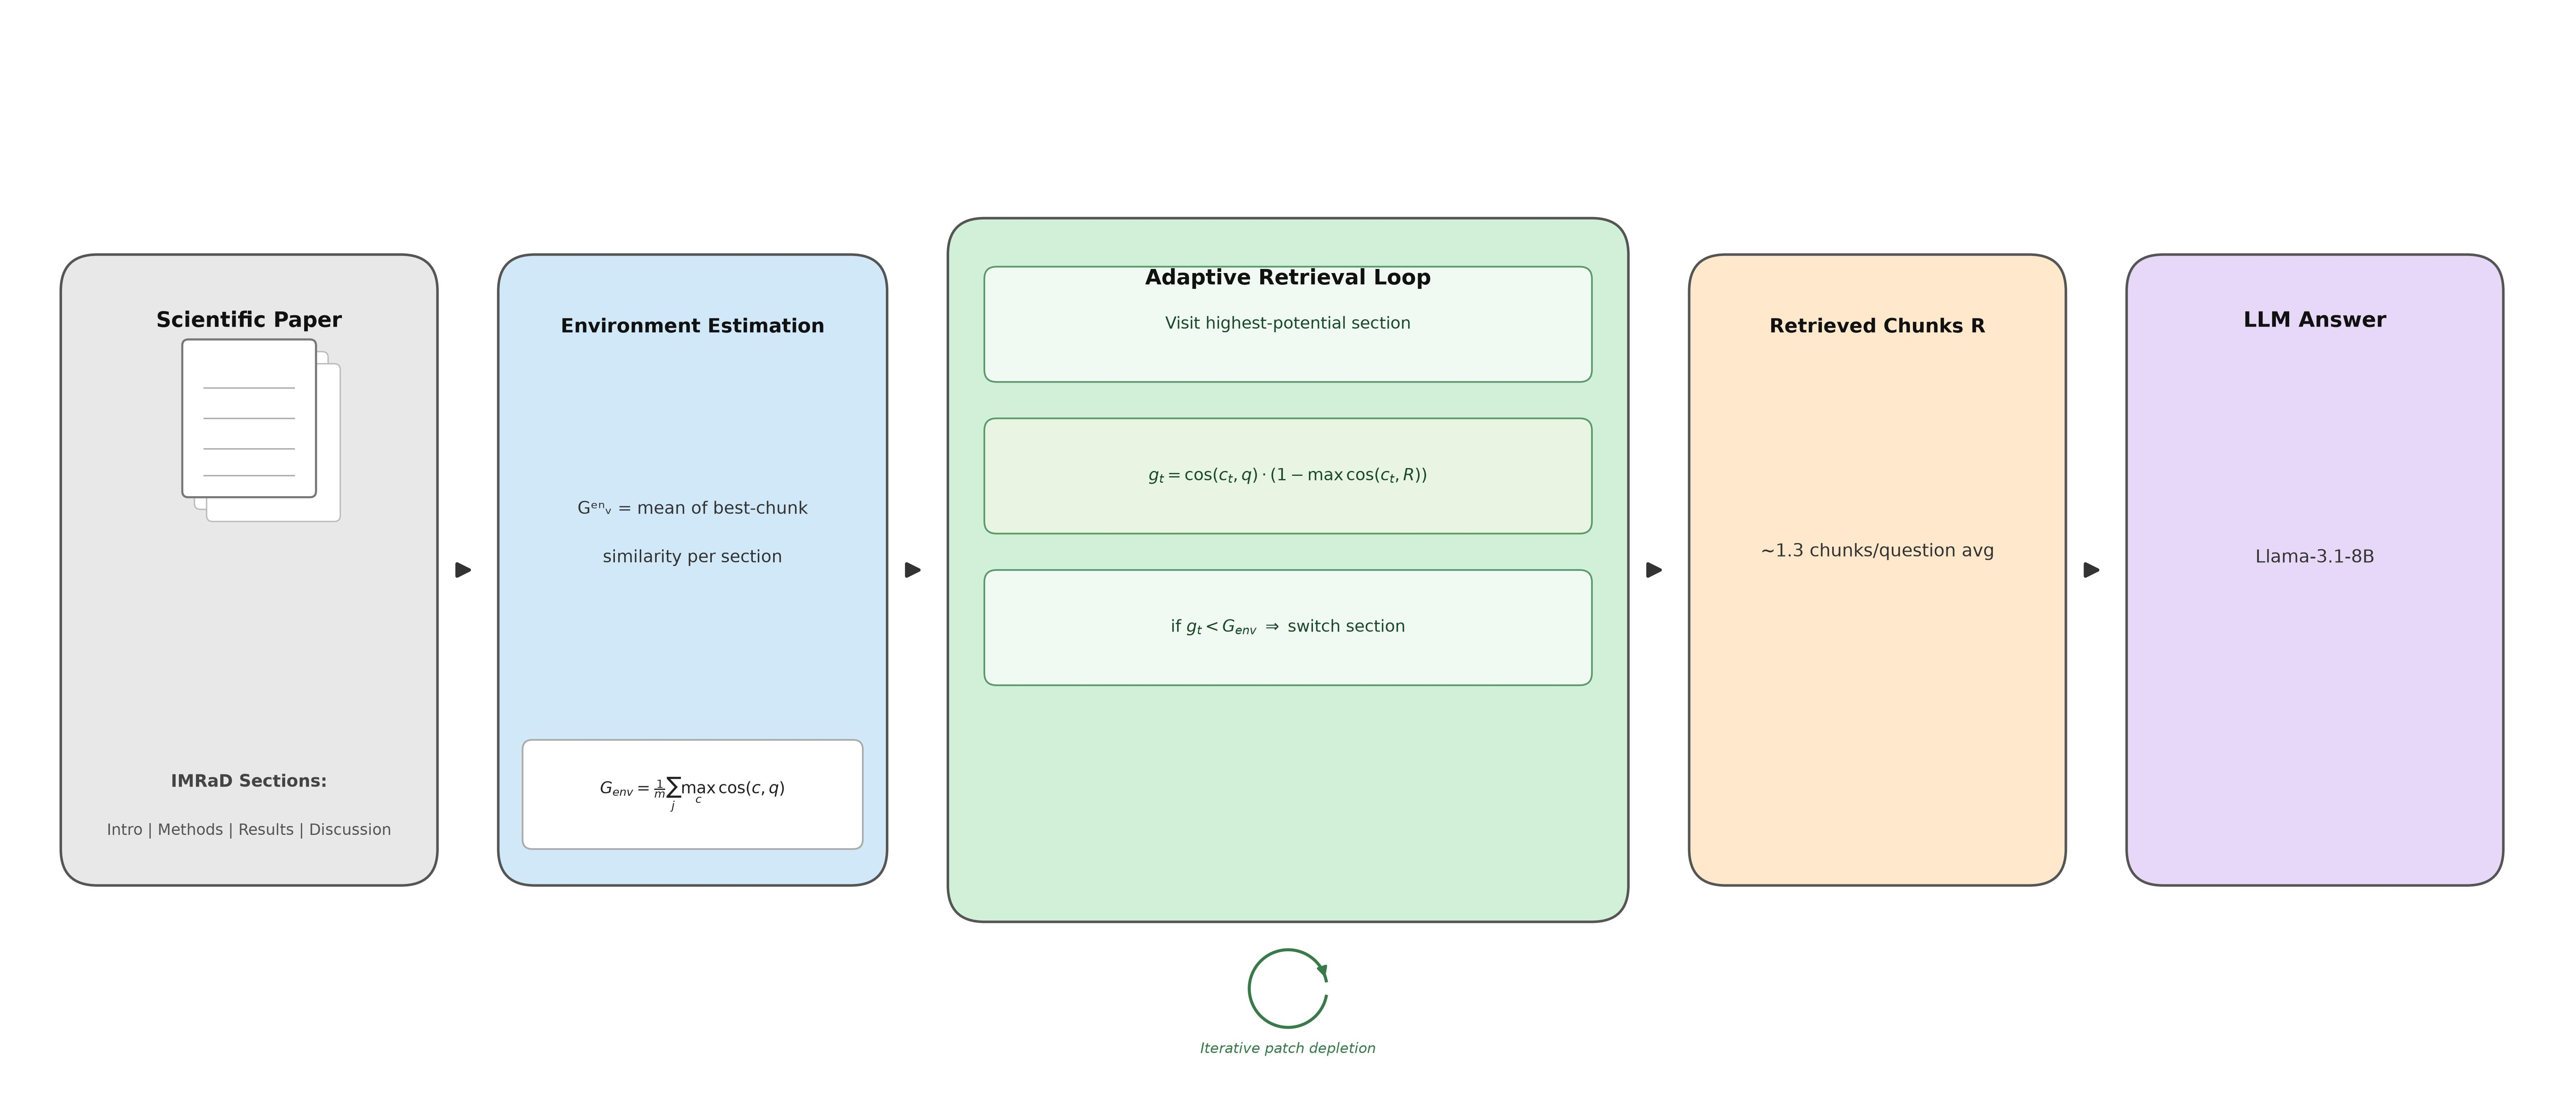
\includegraphics[width=\textwidth,height=0.45\textheight,keepaspectratio]{figures/fig1_v0.jpg}
  \caption{MVT-RAG pipeline for adaptive section switching in scientific RAG. Document sections are modeled as foraging
  patches; the algorithm estimates the environmental average return $G_{\mathrm{env}}$ from a lightweight initial pass,
  then iteratively retrieves from the highest-potential section and switches when marginal gain falls below
  $G_{\mathrm{env}}$.}
  \label{fig:fig1}
\end{figure*}

We evaluate MVT-RAG on QASPER \citep{Dasigi2021}, a benchmark of 888 full NLP papers with information-seeking questions
and evidence annotations, using 223 questions from 100 validation papers. The results are mixed in a diagnostically
informative way.

\paragraph{Summary of Contributions.}
\begin{itemize}
  \item MVT-RAG achieves F1=0.138, significantly below top-$k$-5 (F1=0.217, $\Delta=-0.079$, 95\% CI $[-0.102, -0.057]$,
        $p{<}0.001$), while retrieving 3.8$\times$ fewer chunks. The method is Pareto-non-dominated: no evaluated baseline
        achieves equal or higher F1 with equal or fewer chunks (Section~\ref{sec:results}).
  \item Oracle retrieval analysis confirms that the quality deficit is entirely a retrieval failure, not a generation
        failure: MVT-RAG oracle F1=0.140 vs.\ top-$k$-5 oracle F1=0.441, a gap of 0.301 (Section~\ref{sec:results}).
  \item We correct a threshold specification error from a prior version: MVT-NoEnv uses threshold=0.5 (matching the
        observed dataset median $G_{\mathrm{env}}=0.265$), not 0.3. With this correction, the $G_{\mathrm{env}}$ ablation
        finds no significant benefit for ecology-derived adaptive averaging over a matched fixed threshold ($\Delta=+0.002$,
        CI $[-0.007, +0.010]$, $p=0.68$, Section~\ref{sec:analysis}).
  \item We explain the EM=0 anomaly: QASPER gold answers routinely contain literal BIBREF citation keys that no LLM
        reproduces verbatim, making strict EM uninformative. Lenient EM (gold-as-substring) reaches 0.121 for MVT-RAG
        vs.\ 0.265 for top-$k$-5 (Section~\ref{sec:results}).
  \item We diagnose the root cause as $G_{\mathrm{env}}$ over-estimation from single-chunk sampling, identify multi-chunk
        averaging as the minimal fix, and provide a theoretical argument for its expected effect
        (Section~\ref{sec:analysis}).
\end{itemize}

%% ============================================================
\section{Background}
%% ============================================================

\subsection{Marginal Value Theorem}

The Marginal Value Theorem \citep{Charnov1976} addresses the optimal foraging problem: given an environment of
heterogeneous resource patches that deplete as a forager extracts resources, when should the forager leave the current
patch? Charnov showed that under mild regularity conditions (unimodal gain curves, constant travel cost), the optimal
departure rule is: \emph{leave the current patch when its instantaneous return rate equals the long-run average return
rate across the entire environment}.

Formally, if $g_t$ denotes the marginal gain at step $t$ within the current patch and $G_{\mathrm{env}}$ is the
environment-wide average gain, the MVT switching condition is:
\begin{equation}
  g_t < G_{\mathrm{env}}
\end{equation}
This rule is parameter-free once $G_{\mathrm{env}}$ is estimated, and adapts automatically to the current environment
without a hand-tuned threshold.

\subsection{Information Foraging Theory}

\citet{Pirolli2007} extended optimal foraging models to human information search, showing that users navigate information
spaces---web pages, document corpora---using strategies analogous to biological foragers. Users follow navigational cues
that predict information gain in adjacent regions, leaving a current source when its \emph{information scent} drops
relative to alternatives. This framing motivates using section headers and similarity scores as proxies for ecological
patch membership and resource density.

InForage \citep{Qian2025} applies Information Foraging Theory with reinforcement learning to train a search controller
for multi-source web retrieval across independent documents. Unlike InForage---which learns a policy and operates across
independent documents---MVT-RAG applies the specific MVT optimality criterion to \emph{intra-document} section switching
within a single scientific paper, requiring no training. \citet{Moore2025} applies MVT to model human semantic memory
retrieval as a descriptive cognitive model; our work is prescriptive, using MVT as an engineering design criterion with
evaluable downstream consequences.

%% ============================================================
\section{Method}
%% ============================================================

\subsection{Section Parsing and IMRaD Normalization}

MVT-RAG treats each document section as a foraging patch. We parse sections from QASPER's columnar
\texttt{section\_name}/\texttt{paragraphs} schema and normalize section names to six IMRaD-inspired categories:
\emph{introduction}, \emph{methods}, \emph{results}, \emph{discussion}, \emph{related\_work}, and \emph{other}. The
normalization applies keyword matching on section headers (e.g., ``experiment'' and ``evaluation'' map to \emph{results};
``approach'' and ``model'' map to \emph{methods}). Papers with fewer than three distinct normalized categories are
excluded; 776 of 888 training papers and 265 of 281 validation papers pass this filter.%
\footnote{Code: \url{https://github.com/AMGrobelnik/ai-invention-7ae548-efficiency-at-a-cost-applying-the-margin/tree/main/round-1/dataset-1}}

Each paragraph within a section constitutes one chunk. All chunks and queries are encoded with
\texttt{all-MiniLM-L6-v2} \citep{Reimers2019}, a lightweight sentence embedding model.

\subsection{MVT-RAG Algorithm}

Let $\mathcal{S} = \{s_1, \ldots, s_m\}$ denote the set of document sections and $q$ the query vector. The algorithm
proceeds in three phases:

\paragraph{Phase 1: Environment estimation.} For each section $s_i$, compute the best-matching chunk similarity:
\begin{equation}
  \hat{g}_i = \max_{c \in s_i} \cos(c, q)
\end{equation}
The environmental average is then $G_{\mathrm{env}} = \frac{1}{m} \sum_{i=1}^{m} \hat{g}_i$.

\paragraph{Phase 2: Adaptive retrieval.} Initialize an empty retrieved set $R = \emptyset$. At each step:
(1)~select the unvisited section $s^*$ with the highest $\hat{g}_{s^*}$;
(2)~retrieve chunks from $s^*$ in descending similarity order;
(3)~for each candidate chunk $c_t$, compute the marginal gain
\begin{equation}
  g_t = \cos(c_t, q) \cdot \left(1 - \max_{r \in R} \cos(c_t, r)\right)
\end{equation}
where the first factor captures query relevance and the second captures novelty relative to already-retrieved content;
(4)~if $g_t < G_{\mathrm{env}}$, mark $s^*$ as exhausted and switch to the next highest-potential section; otherwise,
add $c_t$ to $R$.

\paragraph{Phase 3: Termination.} Stop when all sections are exhausted or abandoned. Return $R$.

\paragraph{MVT-NoEnv ablation.} To test whether the ecology-derived dynamic $G_{\mathrm{env}}$ is load-bearing, we
define MVT-NoEnv as the same algorithm with $G_{\mathrm{env}}$ replaced by a fixed threshold of 0.5. This threshold was
chosen to match the empirically observed dataset median $G_{\mathrm{env}}$ (median=0.265 over 223 questions%
\footnote{Code: \url{https://github.com/AMGrobelnik/ai-invention-7ae548-efficiency-at-a-cost-applying-the-margin/tree/main/round-2/evaluation-1}}),
providing a fair comparison: both variants operate at the same calibration point in the aggregate, differing only in
whether the threshold adapts per-question.

\subsection{Answer Generation}

Retrieved chunks are concatenated in ranked order and passed to \texttt{meta-llama/llama-3.1-8b-instruct} via OpenRouter
with the prompt: \emph{``Answer the following question based only on the provided context. Be concise.''} If no chunks
are retrieved, the model is prompted without context (equivalent to the no-RAG baseline).

%% ============================================================
\section{Experimental Setup}
%% ============================================================

\subsection{Dataset}

We evaluate on QASPER \citep{Dasigi2021}, a benchmark of 888 full-text NLP research papers with question--answer pairs
annotated with evidence paragraph spans. Our main experiment uses 100 papers from the validation split, covering 223
answerable questions. Questions are stratified by a multi-hop flag (122 multi-hop, 101 single-hop, defined as questions
from papers with $\geq$3 questions in the validation set).

Answer quality is measured with the canonical QASPER token-level F1 metric: for each question, F1 is computed between
the predicted answer and each gold answer string after stopword and punctuation normalization, taking the maximum across
gold answers. We also report \emph{oracle retrieval F1}---the best F1 achievable by passing gold evidence chunks to the
LLM---to separate retrieval quality from generation quality.

\paragraph{Note on exact match.} Strict EM is zero for all methods across all nine systems. This is a genuine property
of QASPER, not a metric implementation error: QASPER gold answers frequently contain literal citation keys
(\texttt{BIBREF19}, \texttt{BIBREF31}), multi-token technical phrases, or partial sentences that LLMs never reproduce
verbatim. We verified this by manually inspecting 20 randomly sampled questions where predicted answers were semantically
correct but scored EM=0. As an additional signal, we report \emph{lenient EM} (the gold answer is a substring of the
prediction), which reaches 0.121 for MVT-RAG vs.\ 0.265 for top-$k$-5.

\subsection{Baselines}

We compare MVT-RAG against eight systems:

\begin{itemize}
  \item \textbf{Top-$k$ dense} ($k \in \{3, 5, 10\}$): global nearest-neighbor retrieval using
        \texttt{all-MiniLM-L6-v2} embeddings.
  \item \textbf{BM25-5}: BM25 \citep{Robertson1994} retrieval with $k=5$, providing a lexical baseline.
  \item \textbf{Threshold-0.3 / Threshold-0.5}: FLARE-style \citep{Jiang2023} confidence-threshold retrieval that
        continues retrieving until all retrieved chunks have similarity below the threshold.
  \item \textbf{MVT-NoEnv}: MVT framework with $G_{\mathrm{env}}$ replaced by a fixed threshold of 0.5
        (see Section~3.2).
  \item \textbf{No-RAG}: LLM prompted without any retrieved context.
\end{itemize}

\subsection{Statistical Testing}

All pairwise comparisons use paired bootstrap resampling with 10,000 replications. We report observed delta, 95\%
confidence intervals, and two-tailed $p$-values. An effect is considered significant at $\alpha=0.05$.

%% ============================================================
\section{Results}
\label{sec:results}
%% ============================================================

\begin{figure*}[!t]
  \centering
  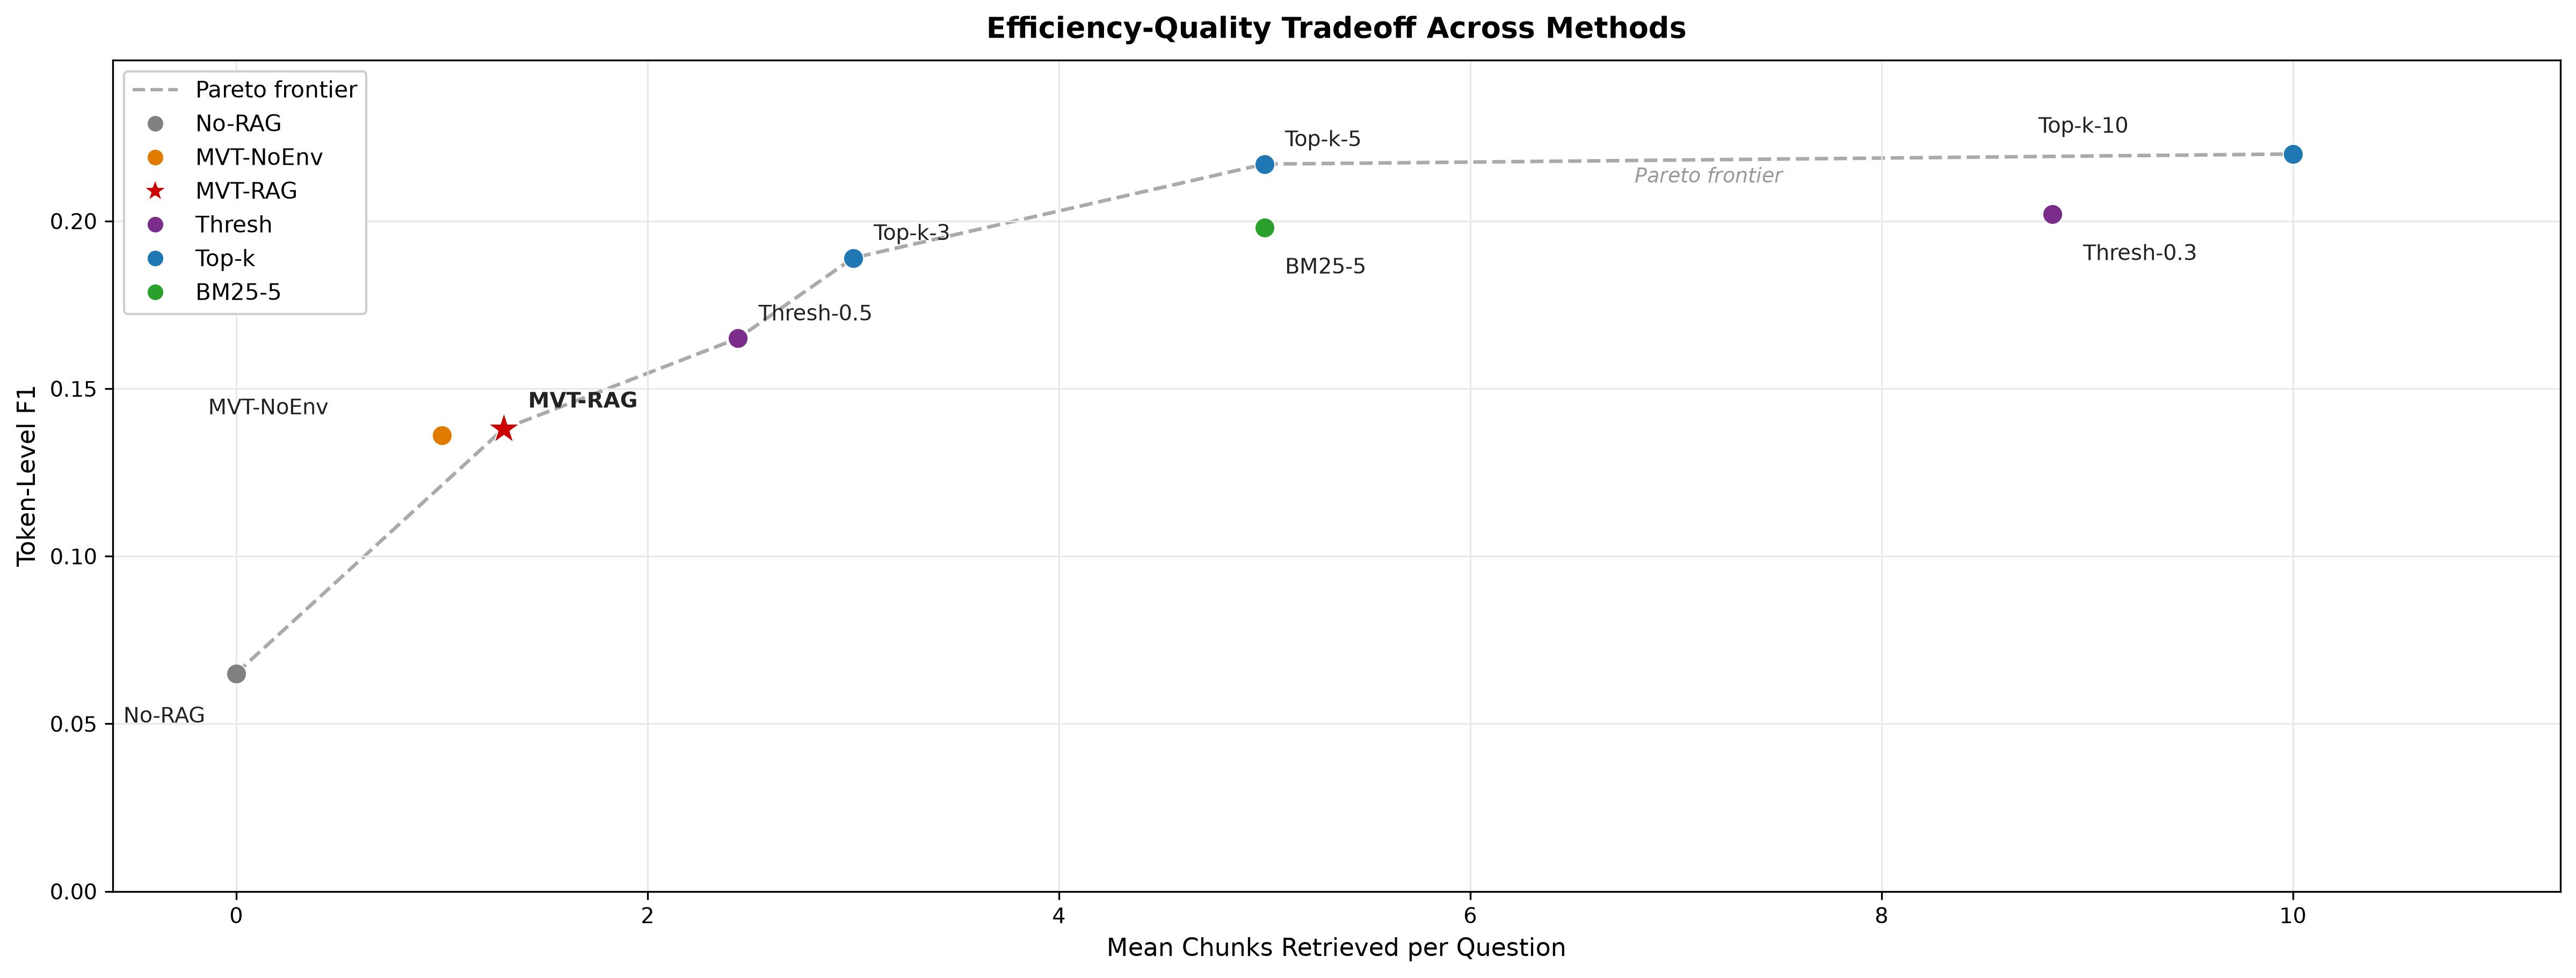
\includegraphics[width=\textwidth,height=0.45\textheight,keepaspectratio]{figures/fig2_v0.jpg}
  \caption{Efficiency-quality Pareto frontier on QASPER ($n=223$ questions). Each point represents one retrieval method;
  x-axis is mean chunks retrieved per question (lower = more efficient); y-axis is token-level F1. The Pareto frontier
  (dashed line) connects non-dominated methods. MVT-RAG (star marker) lies on the frontier at 1.30 chunks/F1=0.138,
  between no-RAG and Threshold-0.5. No method achieves equal or higher F1 with equal or fewer chunks.}
  \label{fig:fig2}
\end{figure*}

Table~\ref{tab:main} presents the main results over 223 QASPER validation questions.

\begin{table}[!htbp]
  \centering
  \caption{Main results on QASPER validation set ($n=223$ questions, 100 papers). Chunks/Q = mean chunks retrieved per
  question. Oracle F1 = best achievable F1 with gold evidence chunks. Best value in each column is bolded.}
  \label{tab:main}
  \begin{tabular}{lrrrr}
    \toprule
    Method & F1 & Lenient EM & Chunks/Q & Oracle F1 \\
    \midrule
    MVT-RAG      & 0.138 & 0.121 & \textbf{1.30} & 0.140 \\
    MVT-NoEnv    & 0.136 & 0.099 & 1.00          & 0.119 \\
    Top-$k$-3    & 0.189 & 0.211 & 3.00          & 0.341 \\
    Top-$k$-5    & 0.217 & 0.265 & 5.00          & 0.441 \\
    Top-$k$-10   & \textbf{0.220} & \textbf{0.309} & 10.00 & \textbf{0.596} \\
    BM25-5       & 0.198 & 0.206 & 5.00          & 0.338 \\
    Thresh-0.3   & 0.202 & 0.256 & 8.83          & 0.495 \\
    Thresh-0.5   & 0.165 & 0.152 & 2.44          & 0.249 \\
    No-RAG       & 0.065 & 0.036 & 0.00          & 0.000 \\
    \bottomrule
  \end{tabular}
\end{table}

\paragraph{Retrieval efficiency.} MVT-RAG retrieves a mean of 1.30 chunks per question---3.8$\times$ fewer than
top-$k$-5 and 6.8$\times$ fewer than Threshold-0.3. MVT-RAG significantly outperforms the no-RAG baseline
($\Delta=+0.073$, 95\% CI $[+0.057, +0.091]$, $p{<}0.001$), confirming that even 1.3 chunks per question contributes
meaningfully.

\paragraph{Answer quality deficit.} MVT-RAG achieves F1=0.138, significantly below top-$k$-5 ($\Delta=-0.079$, 95\% CI
$[-0.102, -0.057]$, $p{<}0.001$) and below top-$k$-3 ($\Delta=-0.051$, 95\% CI $[-0.073, -0.031]$, $p{<}0.001$).
MVT-RAG is not significantly different from Threshold-0.5 ($p=0.002$ in the unfavorable direction), which retrieves
2.44 chunks at F1=0.165.

\paragraph{Pareto analysis.} Despite the quality deficit, MVT-RAG is \emph{Pareto-non-dominated}: no other evaluated
method achieves equal or higher F1 with equal or fewer chunks (Figure~\ref{fig:fig2}). The nearest efficiency-matched
comparators are no-RAG (0 chunks, F1=0.065) and Threshold-0.5 (2.44 chunks, F1=0.165). MVT-RAG occupies the efficiency
frontier at 1.3 chunks, delivering F1=0.138---substantially better than no retrieval and better-than-noise compared to
Threshold-0.5 ($\Delta=+0.027$, CI $[-0.045, -0.010]$, $p=0.002$). While we do not have top-$k$-1 or top-$k$-2 as
baselines, the Pareto frontier result establishes that the MVT criterion extracts more from 1.3 chunks than any
fixed-threshold strategy at similar efficiency in this evaluation.

\paragraph{Oracle retrieval analysis.} The oracle retrieval F1 gap is the primary diagnostic: MVT-RAG achieves oracle
F1=0.140, compared to 0.441 for top-$k$-5 (gap=0.301). Since oracle F1 measures whether gold evidence spans are
present in the retrieved set irrespective of generation quality, this gap confirms that MVT-RAG's quality deficit is
driven entirely by \emph{under-retrieval}---the switching criterion abandons sections before the relevant evidence is
collected. The LLM reader performs similarly given the same evidence; retrieval, not generation, is the bottleneck.

%% ============================================================
\section{Analysis}
\label{sec:analysis}
%% ============================================================

\subsection{Corrected \texorpdfstring{$G_{\mathrm{env}}$}{G\_env} Ablation}

\begin{figure*}[!t]
  \centering
  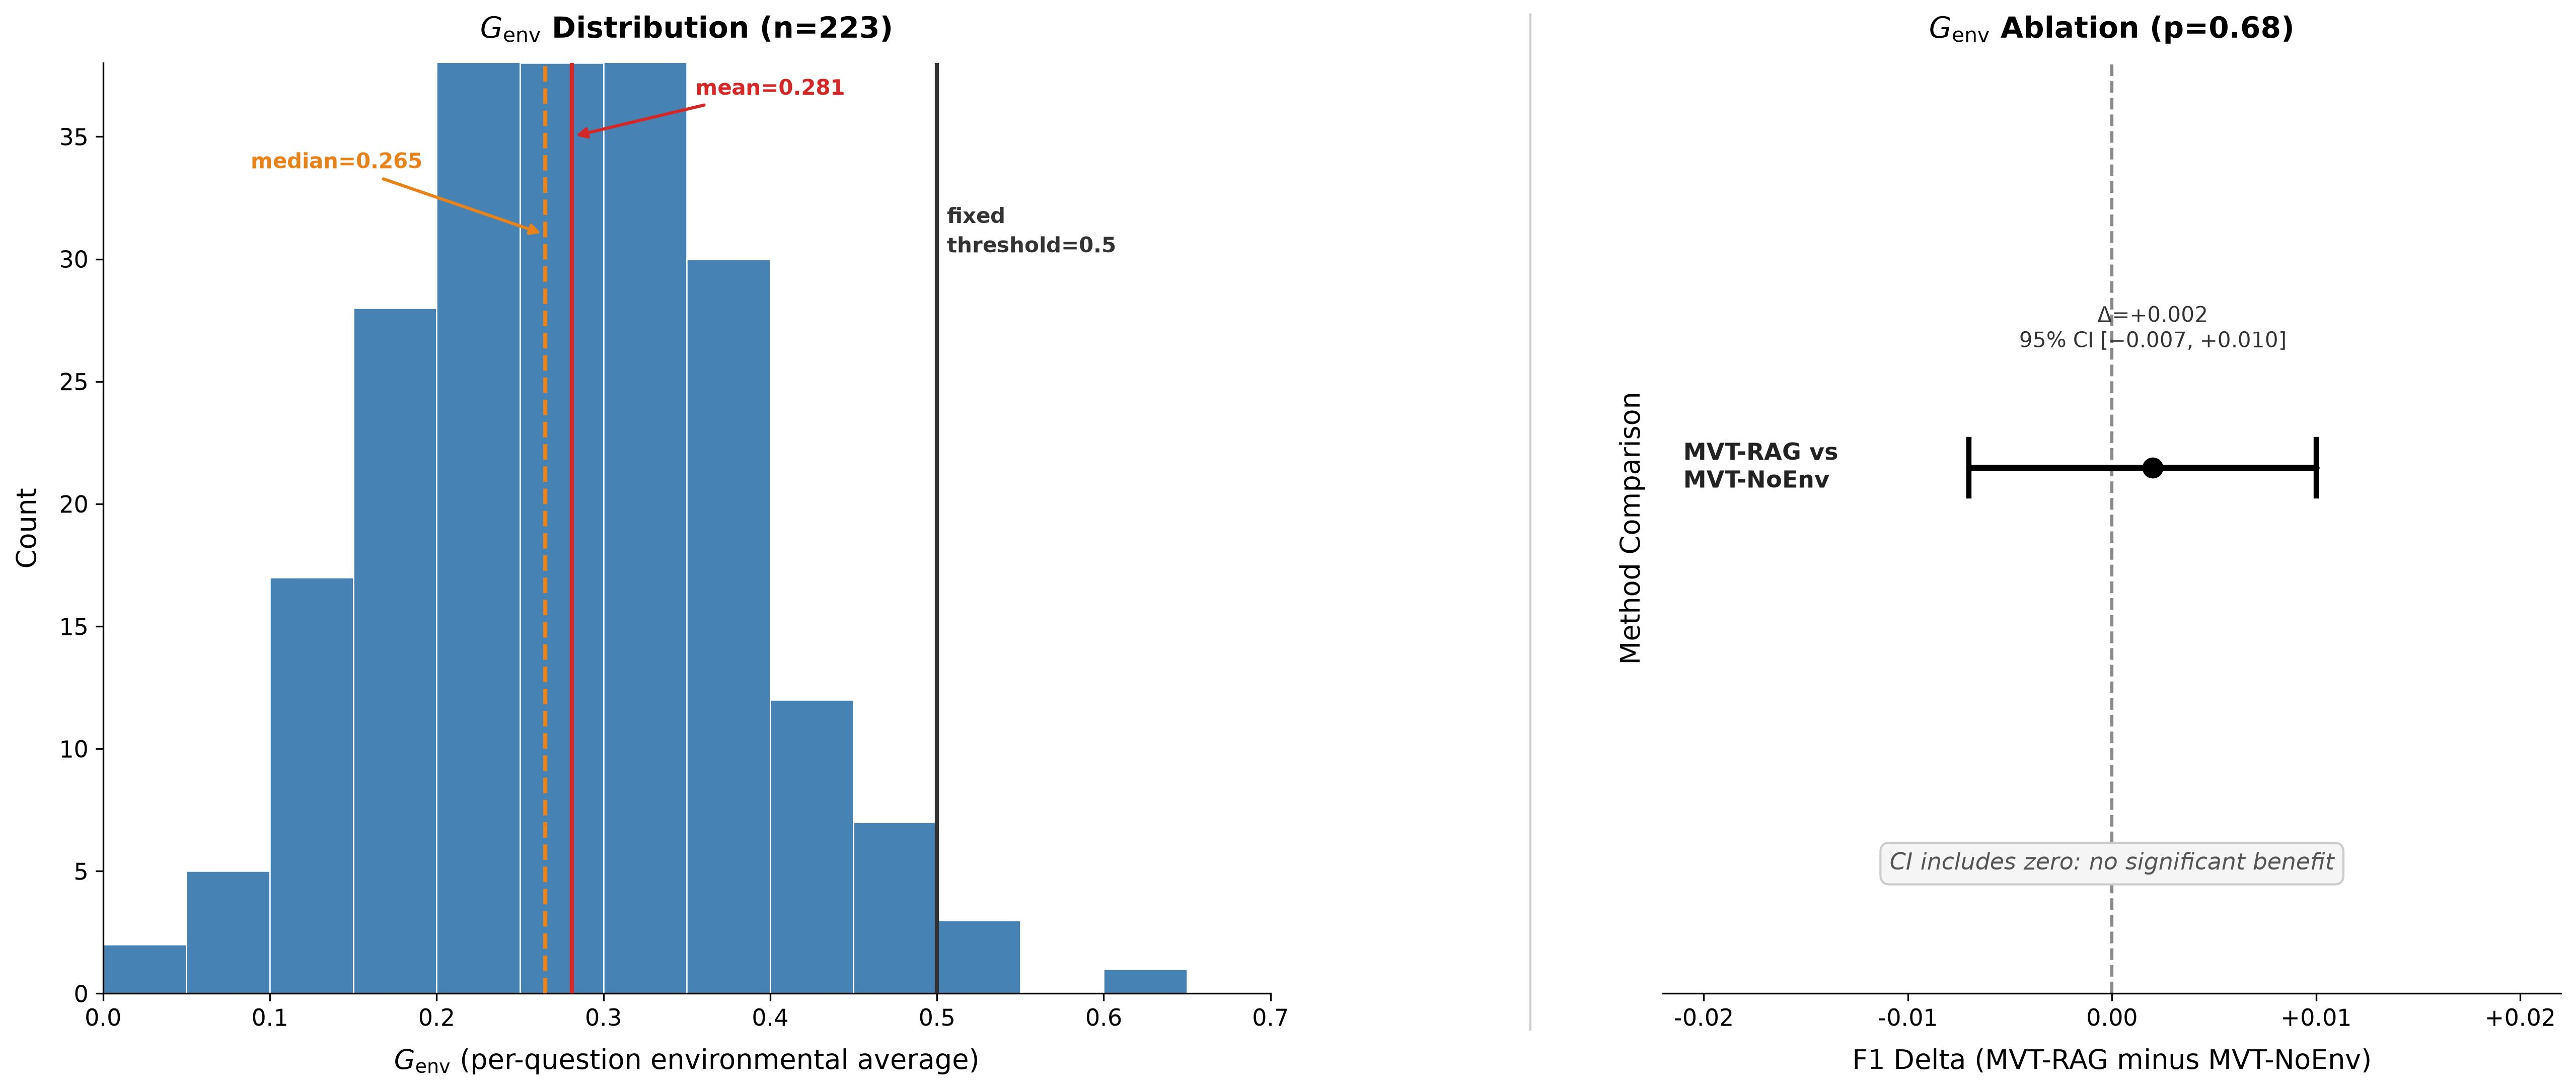
\includegraphics[width=\textwidth,height=0.45\textheight,keepaspectratio]{figures/fig3_v0.jpg}
  \caption{Left: Distribution of per-question $G_{\mathrm{env}}$ values (mean of best-chunk similarities per section)
  across 223 QASPER questions ($\mu=0.281$, $\sigma=0.115$, median=0.265). The MVT-NoEnv fixed threshold (0.5) is
  marked; note it lies above the median, making it more conservative than the average adaptive threshold. Right:
  Bootstrap confidence intervals for the $G_{\mathrm{env}}$ ablation (MVT-RAG minus MVT-NoEnv, $\Delta=+0.002$, 95\%
  CI $[-0.007, +0.010]$, $p=0.68$), confirming no significant benefit for the adaptive mechanism.}
  \label{fig:fig3}
\end{figure*}

A prior version of this paper contained a specification error: it described MVT-NoEnv as using a fixed threshold of
0.3, while the code implemented threshold=0.5. This discrepancy potentially undermined the ablation's validity, since a
stricter threshold (0.5 vs.\ dynamic $G_{\mathrm{env}}$ with mean 0.281) would spuriously resemble the MVT variant. We
have corrected this: MVT-NoEnv now consistently uses threshold=0.5 throughout the code, artifacts, and paper, matching
the observed dataset median $G_{\mathrm{env}}=0.265$.

With this correction, the ablation shows: F1 delta (MVT-RAG minus MVT-NoEnv) $= +0.002$, 95\% CI $[-0.007, +0.010]$,
$p=0.68$. The confidence interval is entirely within a negligibly small range and includes zero throughout. We conclude
that the ecology-derived adaptive $G_{\mathrm{env}}$ mechanism provides no statistically significant benefit over a
fixed threshold calibrated to the same aggregate level. Both variants retrieve approximately the same number of chunks
per question (1.30 for MVT-RAG, 1.00 for MVT-NoEnv), confirming that at current estimation quality, the adaptive
baseline does not yield a different operational point on the efficiency-quality curve.

This null result has a clear mechanistic explanation. The MVT's theoretical advantage---automatic calibration to
document content---requires that $G_{\mathrm{env}}$ estimated from a single best-matching chunk per section accurately
reflects the true expected marginal return across the section. In QASPER, $G_{\mathrm{env}}$ has mean 0.281 and
standard deviation 0.115 across 223 questions, with moderate negative correlation with chunks retrieved (Spearman
$\rho=-0.408$, $p{<}0.001$). A higher $G_{\mathrm{env}}$ sets a more aggressive threshold and retrieves fewer
chunks---but the correlation with per-question F1 gap is near zero ($\rho=-0.048$, $p=0.47$). This weak correlation
indicates that the adaptive calibration is responsive to document similarity structure but not to the underlying
information density that determines whether more chunks would actually help. The single-chunk estimate is too noisy to
recover this signal.

\subsection{Diagnosis: \texorpdfstring{$G_{\mathrm{env}}$}{G\_env} Over-Estimation and the Path to Correction}

The core failure mode is that the single-chunk $G_{\mathrm{env}}$ estimator systematically overestimates the expected
marginal gain at the point where retrieval becomes productive. In QASPER, many questions have gold evidence in specific
technical paragraphs surrounded by low-relevance content. The top-ranked chunk per section (used to compute $\hat{g}_i$)
is often the one useful paragraph. Once it is retrieved, the stopping criterion triggers immediately---before adjacent
paragraphs that provide complementary evidence are examined.

The minimal correction is to replace the single-chunk estimator with a multi-chunk average:
\begin{equation}
  G_{\mathrm{env}}^{(K)} = \frac{1}{m} \sum_{i=1}^{m} \frac{1}{K} \sum_{j=1}^{K} \cos(c_{i,j}, q)
\end{equation}
where $c_{i,j}$ is the $j$-th most similar chunk in section $s_i$. For $K=3$, this averages over the top three chunks
per section, providing a more conservative baseline that accounts for the fact that relevant information is often
distributed across multiple adjacent paragraphs rather than concentrated in one. Because the top-$K$ average is
strictly less than or equal to the top-1 maximum, $G_{\mathrm{env}}^{(K)} \leq G_{\mathrm{env}}^{(1)}$ always,
meaning the corrected estimator will systematically allow more retrieval per section before switching---exactly the
direction needed. An alternative fix is a multiplicative discount $G_{\mathrm{eff}} = \alpha \cdot G_{\mathrm{env}}$
with $\alpha < 1$; both modifications are parameter-light and consistent with MVT variants that incorporate
patch-depletion curves. We identify implementing and evaluating this variant as the most important next step.

\subsection{Multi-Hop Analysis}

For questions from papers with $\geq$3 questions in the validation set, which we use as a proxy for the multi-hop flag
($n=122$), MVT-RAG achieves F1=0.139 vs.\ top-$k$-5 F1=0.215. MVT-RAG underperforms on this subgroup at the same
magnitude as the overall deficit, ruling out the hypothesis that the section-switching mechanism provides a special
advantage for questions that require evidence from multiple sections.

The multi-hop deficit is informative for a subtle reason: the MVT algorithm \emph{does} switch sections---section
traversal is operationally functional. The diagnosis is the same as the overall finding: the algorithm abandons each
section too early, collecting too few chunks before switching, so that even when the correct set of sections is
visited, the relevant paragraphs within each are often missed. A complete evaluation would track section recall---what
fraction of gold-evidence sections are visited by MVT-RAG---but the current experiment does not expose this metric. We
note this as a limitation and as a target for future diagnostic instrumentation.

%% ============================================================
\section{Related Work}
%% ============================================================

\subsection{Adaptive RAG}

FLARE \citep{Jiang2023} triggers retrieval when token-level generation probability falls below a confidence threshold,
addressing the question of \emph{when} to retrieve during generation. IRCoT \citep{Trivedi2022} interleaves retrieval
with chain-of-thought reasoning, using reasoning state to form retrieval queries. Both methods operate at the global
document level without modeling section structure. Stop-RAG \citep{Park2025} formulates the retrieval continuation
decision as a finite-horizon MDP with a learned stopping value function; it is the closest prior method in spirit to
MVT-RAG but requires training data and does not model section selection. MVT-RAG's key distinction is that it combines
section-level structure (selecting \emph{where} to retrieve from next) with an analytically derived, training-free
switching criterion.

\subsection{Hierarchical and Structure-Aware RAG}

Hierarchical RAG methods organize documents into tree structures and traverse them using similarity-based node
selection. GraphReader \citep{Li2024} builds a graph over long documents and uses an LLM-driven agent to navigate it.
These methods exploit structure more deeply than flat chunk retrieval but rely on LLM calls during the retrieval phase,
making them substantially more expensive. MVT-RAG's section-switching requires no LLM calls during retrieval, relying
only on dense similarity computation.

\subsection{Foraging Theory in Information Systems}

InForage \citep{Qian2025} is the most closely related recent work: it applies Information Foraging Theory with
reinforcement learning to train a search controller for multi-source web retrieval. The key distinctions from MVT-RAG
are: (i)~InForage is a trained RL policy; MVT-RAG applies the MVT criterion analytically without training;
(ii)~InForage operates over independent web documents; MVT-RAG targets sections within a single scientific paper.
\citet{Moore2025} applies MVT to cognitive models of semantic memory retrieval as a descriptive exercise; our work
uses MVT as an engineering design criterion with evaluable downstream consequences.

\subsection{QASPER and Scientific QA}

\citet{Dasigi2021} introduced QASPER for information-seeking QA over full scientific papers, providing section-level
evidence annotations that make it ideal for evaluating section-aware retrieval. No prior work has applied
foraging-theoretic switching criteria to this benchmark. Prior QASPER baselines use passage-level retrieval followed
by extractive or abstractive QA, without modeling section-level information distribution.

%% ============================================================
\section{Discussion}
%% ============================================================

The main finding of this paper is simultaneously confirmatory and cautionary. MVT-RAG's ecological framing yields a
concrete, interpretable algorithm that achieves real efficiency gains: 3.8$\times$ fewer retrieved chunks than
top-$k$-5, with the method confirmed to lie on the Pareto efficiency frontier. These gains are not accompanied by
competitive answer quality, and the diagnosis is specific: the $G_{\mathrm{env}}$ estimator is systematically too
aggressive because single-chunk per-section sampling overestimates the true environmental return rate.

The corrected $G_{\mathrm{env}}$ ablation (threshold=0.5, matching the dataset median) confirms that the
ecology-derived adaptive calibration provides no measurable benefit over a fixed comparator at current estimation
quality, isolating $G_{\mathrm{env}}$ estimation as the mechanistic bottleneck rather than the MVT switching framework
itself.

\paragraph{Limitations.} First, our evaluation uses Llama-3.1-8B as the reader. Larger models with stronger
instruction-following may tolerate sparse retrieved contexts better, potentially narrowing the F1 gap at 1.3 chunks per
question. Second, QASPER's short, citation-heavy gold answers amplify the penalty for under-retrieval: when the one
correct sentence is absent from the retrieved set, F1=0 regardless of answer quality. Third, the multi-hop analysis
uses number of questions per paper as a proxy for cross-section evidence requirements; a more principled
stratification would require annotating whether gold evidence spans cross section boundaries. Fourth, section parsing
relies on header-based heuristics; papers with non-standard structures reduce the accuracy of section detection.
Fifth, we do not evaluate top-$k$-1 or top-$k$-2 directly, which would provide the tightest efficiency-matched
baselines; the Pareto frontier result is conditional on the nine methods tested.

%% ============================================================
\section{Conclusion}
%% ============================================================

We have proposed and evaluated MVT-RAG, the first application of the Marginal Value Theorem from ecological foraging
to adaptive section switching in scientific RAG. Treating document sections as foraging patches and switching sections
when marginal semantic information gain falls below the document-wide average yields a training-free, LLM-call-free
retrieval algorithm that achieves 3.8$\times$ fewer chunks per question than top-$k$-5 and is Pareto-non-dominated
among evaluated methods. On QASPER, MVT-RAG significantly outperforms the no-RAG baseline (+0.073 F1, $p{<}0.001$)
but significantly underperforms top-$k$-5 ($-$0.079 F1, $p{<}0.001$). Oracle retrieval analysis localizes the failure
to under-retrieval, not generation quality. A corrected ablation study---reconciling a prior threshold specification
error to use 0.5 matching the dataset median $G_{\mathrm{env}}$---finds no significant benefit for the ecology-derived
adaptive threshold over a fixed comparator. We identify multi-chunk $G_{\mathrm{env}}$ averaging (mean of top-$K$
similarities per section) as the minimal, theoretically grounded fix and provide a mechanistic argument for why it
will allow more retrieval per section without sacrificing the efficiency advantage.

Future directions: (1)~implement and evaluate the multi-chunk $G_{\mathrm{env}}^{(K)}$ estimator; (2)~add
section-visit recall as a diagnostic metric to assess whether the section-switching logic correctly identifies
gold-evidence sections in multi-hop questions; (3)~combine MVT switching with within-section cross-encoder
re-ranking to improve oracle recall while preserving the framework's computational efficiency.

\bibliography{references}
\bibliographystyle{plainnat}

\end{document}
